% ICICT 2027 (Springer LNNS) -- ANONYMIZED REVIEW VERSION (double-blind).
% Build: latexmk -pdf main.tex   (needs llncs.cls; included in TeX Live/MacTeX, or https://ctan.org/pkg/llncs)
% Camera-ready: restore authors/affiliations, repository URL and DOI (search for CAMERA-READY).
\documentclass[runningheads]{llncs}
\usepackage[T1]{fontenc}
\usepackage{graphicx}
\usepackage{amsmath,amssymb}
\usepackage{booktabs}
\usepackage{array}
\newcolumntype{L}[1]{>{\raggedright\arraybackslash}p{#1}}
\usepackage{multirow}
\usepackage{xcolor}
\usepackage[hidelinks]{hyperref}
\hypersetup{pdfauthor={},pdftitle={},pdfsubject={},pdfkeywords={},pdfcreator={},pdfproducer={}}
\setlength{\emergencystretch}{1.5em}
\newcommand{\todo}[1]{\textcolor{red}{[TODO: #1]}}

\begin{document}

\title{When Do Census Bureau Geocodes Land in the Wrong Tract? Error Direction, Block-Face Matching and Abstention Rules}
\titlerunning{When Do Census Bureau Geocodes Land in the Wrong Tract?}
% CAMERA-READY: replace with real author block
\author{Anonymous Author(s)}
\authorrunning{Anonymous}
\institute{Affiliation omitted for double-blind review}

\maketitle

\begin{abstract}
Agencies assign geocoded addresses to census tracts with a point-in-polygon test that returns one label even near a boundary. We compare U.S.\ Census Bureau geocodes with independent reference address points in New York City, Utah and 18 sampled counties. Displacements are large (median 19--86\,m), yet among 5{,}971 addresses near tract lines only 0.04--2.0\% fall in another tract, against 10.8--20.2\% for the same displacement lengths in random directions, a gap that survives counting every excluded match as an error and holds for block groups and blocks. Using the street edge and side the geocoder reports, the tract was wrong for 2 of 5{,}594 addresses whose reference point lies on the matched block face, against 42 of 293 elsewhere: errors come from matching the wrong block face, not from positional spread. Boundary distance flags them poorly; a changed street direction or house number in the matched address flagged 12 of the 44 errors at a 4.6\% review share, against 5 for distance. Eight of the wrong tracts changed HUD Qualified Census Tract status. A 13{,}000-location simulation shows where isotropic error models and distance rules apply.
\keywords{Geocoding \and Positional uncertainty \and Point-in-polygon \and Census tracts \and Selective prediction}
\end{abstract}

%=====================================================================
\section{Introduction}
Many digital public services geocode an address and assign the coordinate to an administrative area by a point-in-polygon (PIP) test. That label decides which tract a disease case is counted in, whether a household lies in a qualifying area (e.g., HUD Qualified Census Tracts for the Low-Income Housing Tax Credit), and which neighbourhood statistics a record feeds. A geocode on the ``wrong side of the tract'' biases area-based measures~\cite{krieger2001,krieger2002,rushton2006}.

The PIP step is \emph{silent}: geocodes are displaced by tens of metres~\cite{cayo2003,zandbergen2008,zandbergen2009}, yet GIS software returns one label with no sign that the point lies near a boundary. A common response is to model positional error as isotropic and flag points within an error radius of a boundary. We ask whether that model describes a real geocoder, and what does. Our contributions are:
\begin{enumerate}
\item \textbf{Multi-region evidence} for the U.S.\ Census Bureau geocoder in New York City, Utah and 18 sampled counties, with direction-only counterfactuals (same displacement length; random, along-street or across-street direction), sensitivity to excluded matches, and a test using the street edge and side the geocoder itself matched (Sect.~\ref{sec:real}).
\item \textbf{Operational findings}: boundary distance flags the remaining errors poorly, the geocoder's own match details flag them better, some errors change program eligibility (HUD Qualified Census Tracts), and generalized boundary files add avoidable error.
\item \textbf{A simulation baseline}: 13{,}000 locations at three administrative levels with 520{,}000 noisy observations, showing where the isotropic model holds, how abstention rules compare at matched risk, and how thresholds transfer to held-out states (Sect.~\ref{sec:sim}).
\end{enumerate}
That street geocodes usually keep the correct tract is known~\cite{whitsel2006,brokamp2018,kinnee2020}; we explain why, identify which errors remain and how to flag them. The crossing formulas and the bounded-error distance rule are standard geometry; we show where they hold and how poorly they describe a real national geocoder.

%=====================================================================
\section{Related Work}
\textbf{Geocoding error and area assignment.} Geocoding errors range from metres to hundreds of metres and grow in rural areas~\cite{goldberg2007,cayo2003,zandbergen2008,zandbergen2009}, follow non-normal distributions~\cite{zandbergen2008b}, and in rural Iowa formed a cross-shaped, street-aligned pattern~\cite{zimmerman2007}; error angles in Atlanta appeared uniform~\cite{strickland2007}, and in New York City street-segment geocodes were displaced mostly toward one direction~\cite{kinnee2020}. Match rates also differ by geography~\cite{oliver2005}. Consequences for health studies are reviewed in~\cite{rushton2006,jacquez2012}. Krieger et al.~\cite{krieger2001} and Whitsel et al.~\cite{whitsel2006} measured tract misassignment by commercial geocoders (concordance 85--98\%), Brokamp et al.~\cite{brokamp2018} found 95.5\% tract accuracy for a TIGER range geocoder, HUD geocodes of tax-credit housing were in the wrong tract for 3.3\% of developments~\cite{wilson2024}, Goldberg and Cockburn~\cite{goldberg2012} showed that administrative boundaries and geocoding error change cancer rates, Kinnee et al.~\cite{kinnee2020} found few differences between geocoding methods in census-area assignment, and Berg et al.~\cite{berg2026} describe records joined to implausible census blocks. We add counterfactuals that keep each measured displacement length and change only its direction, and a test on the geocoder's own matched street edge.

\textbf{Spatial uncertainty and point-in-polygon.} Uncertainty in GIS has a long tradition~\cite{heuvelink1998,shi2010}. Epsilon bands around lines~\cite{perkal1958} and their use to classify points as definitely or possibly inside a polygon~\cite{blakemore1984} underlie the distance rule we evaluate; probability-based PIP integrates a positional error distribution over the polygon~\cite{cheung2004}. We compare rules by the risk--coverage trade-off of selective prediction~\cite{chow1970,geifman2017} and by calibration~\cite{guo2017}.

%=====================================================================
\section{Problem and Isotropic Risk Model}\label{sec:model}
\textbf{Task.} Let $\mathcal{R}$ be a set of non-overlapping polygons (tracts, ZCTAs or counties) that need not cover all land and water. A true location $x$ has reference label $r(x)$, or is unassigned. A system observes $\tilde x = x + e$ with error scale $R$ (the maximum radius for bounded error, else the 95\% radius) and answers or abstains (another region is plausible, or the error disk reaches area outside every polygon). $d_{\mathrm{true}}=\operatorname{dist}(x,\partial r(x))$ stratifies the benchmark; $d_{\mathrm{obs}}=\operatorname{dist}(\tilde x,\partial r(\tilde x))$ is the only distance available in practice.

\textbf{Straight-boundary model.} For a straight boundary and isotropic error only the across-boundary component matters. For error uniform in a disk of radius $R$ and $u=d_{\mathrm{true}}/R<1$,
\begin{equation}
P_{\mathrm{uni}}(u) = \tfrac{1}{\pi}\left(\arccos u - u\sqrt{1-u^2}\right),\qquad P_{\mathrm{uni}}=0 \text{ for } u\ge 1; \label{eq:uni}
\end{equation}
for Gaussian error with $\sigma=R/2.4477$, $P_{\mathrm{gau}}=\Phi(-d_{\mathrm{true}}/\sigma)$, and for isotropic error with displacement lengths $\rho_1,\dots,\rho_n$,
\begin{equation}
P(d_{\mathrm{true}})=\frac{1}{n}\sum_{i:\,\rho_i>d_{\mathrm{true}}}\frac{\arccos(d_{\mathrm{true}}/\rho_i)}{\pi}. \label{eq:emp}
\end{equation}
Simulations drawn from these models must reproduce these formulas on straight boundaries, so agreement there checks the implementation; the informative quantities are departures at complex geometry and the transfer to real geocodes. Eq.~(\ref{eq:emp}) with measured displacement lengths is also the random-direction baseline of Sect.~\ref{sec:real}.

\textbf{Strategies.} All see only $\tilde x$ and $R$. \emph{Crisp PIP} returns the containing region. The \emph{distance rule} answers if $d_{\mathrm{obs}}\ge\tau$ (default $\tau=R$); under \emph{bounded} error the answer is then certain. \emph{Monte Carlo} (MC) uses $N$ error draws (default 100); the \emph{disk overlay} returns region area fractions within radius $R$ (exact for uniform error); the \emph{Gaussian overlay} integrates the Gaussian density (radial Gauss--Legendre, 24 nodes on $[0,5\sigma]$). Probabilistic strategies answer if the top probability is $\ge\theta$ (default 0.9); mass outside all polygons stays unassigned. An answer is wrong when its label (unassigned counts as a label) differs from the reference label.

%=====================================================================
\section{Simulation Benchmark}\label{sec:bench}\label{sec:sim}
\textbf{Design.} 13{,}000 true locations in the 50 states and D.C.\ (4{,}000 county, 4{,}000 ZCTA, 5{,}000 tract) on TIGER/Line 2025 boundaries~\cite{tiger2025}, stratified by $d_{\mathrm{true}}$ (0--10, 10--100, 100--500, $\ge$500\,m). Each receives $K=5$ observations in eight settings (uniform or Gaussian $\times$ $R\in\{5,10,20,50\}$\,m): 520{,}000 observations. A separately sampled stress set (4{,}907 locations at corners, junctions and slivers, 20 observations each at $R$=20 and 50\,m) and heavy-tailed runs (Student-$t_3$, contaminated Gaussian, log-normal) are not part of these. All distances are computed in EPSG:2163 (US National Atlas Equal Area, now EPSG:9311); at our real-data reference points its linear scale error is at most 1.6\% and its angular distortion at most 2.1$^\circ$. CIs come from a bootstrap over locations (thresholds re-selected in every replicate).

\textbf{Where the isotropic model holds.} Observed crossing rates match Eq.~(\ref{eq:uni}) and its Gaussian analogue (observed/predicted 0.988 and 0.994), as they must; the empirical form holds for each heavy-tailed model. Under uniform error with $R$=20\,m, crisp PIP misassigns 34.3\% [33.2, 35.5] of observations within 10\,m of a boundary and none beyond $R$. The non-trivial finding is local geometry: junctions (1.14--1.19), corners (1.13--1.20) and slivers (1.06--1.21) exceed the straight-boundary prediction by 6--21\% (CIs exclude 1 in 11 of 12 cases).

\begin{table}[t]
\centering
\caption{Coverage (\%) at matched risk targets, benchmark pooled over levels; 0 = target not reached. Bootstrap 95\% CIs extend at most 1.5 points, except MC at Gaussian 50\,m, 0.1\% ([0, 79.0]). Runtime: ms per 1{,}000 queries at $R$=20\,m, single process, Apple M4 Pro, Python 3.11, Shapely 2.2.}
\label{tab:strategies}
\small\setlength{\tabcolsep}{2.2pt}
\begin{tabular}{lrrrrrrrrr}
\toprule
& \multicolumn{2}{c}{Unif.\ 20\,m} & \multicolumn{2}{c}{Gauss.\ 20\,m} & \multicolumn{2}{c}{Unif.\ 50\,m} & \multicolumn{2}{c}{Gauss.\ 50\,m} & \\
Strategy & 0.5\% & 0.1\% & 0.5\% & 0.1\% & 0.5\% & 0.1\% & 0.5\% & 0.1\% & ms/1k \\
\midrule
Distance rule & 91.7 & 89.5 & 92.4 & 88.7 & 82.2 & 79.6 & 83.7 & 78.4 & 5 \\
Disk overlay & 91.7 & 89.5 & 92.4 & 88.7 & 82.3 & 79.6 & 83.8 & 78.3 & 13 \\
Gaussian overlay & 91.7 & 89.5 & 92.4 & 88.7 & 82.3 & 79.6 & 83.8 & 78.3 & 500 \\
MC ($N$=100) & 91.6 & 89.3 & 92.3 & 88.8 & 81.7 & 78.7 & 83.2 & 0 & 67 \\
\bottomrule
\end{tabular}
\end{table}

\textbf{Abstention at matched risk.} On a straight boundary an overlay centred on $\tilde x$ is a monotone function of $d_{\mathrm{obs}}$, so the two rank queries identically; they can differ only at complex geometry, which is too rare in the benchmark to change the ranking. Accordingly, in all 24 combinations of 8 error settings and targets of 1, 0.5 and 0.1\% (Table~\ref{tab:strategies} shows four settings at two targets), the distance rule's coverage is within 0.1 points of both overlays at a fraction of the cost; MC is up to 0.9 points lower and cannot reach 0.1\% at Gaussian 50\,m. On the stress set the distance rule ranks better at corners and slivers, overlays only at water edges. Overlays are not calibrated posteriors here: they assume a flat prior on $x$, and the benchmark over-samples boundaries. These conclusions cover the tested overlays under this sampling design. Under heavy tails the distance rule still reached 67.9\% coverage at risk $\le$0.1\% (Student-$t_3$, $R$=50\,m), the disk overlay none.

\begin{table}[t]
\centering
\caption{Held-out states, distance rule, target 0.1\%, location-adjusted Wilson threshold: errors/answered per held-out fold (folds are groups of states of unequal size; 65{,}000 observations per setting) and pooled coverage; $R$=5 and 10\,m in the repository.}
\label{tab:folds}
\small\setlength{\tabcolsep}{3pt}
\begin{tabular}{lrrrrrr}
\toprule
Setting & Fold 1 & Fold 2 & Fold 3 & Fold 4 & Fold 5 & Cov.\,\% \\
\midrule
Uniform 20\,m & 4/17{,}387 & 5/11{,}918 & 0/9{,}611 & 5/10{,}835 & 3/7{,}902 & 88.7 \\
Uniform 50\,m & 4/15{,}429 & 3/10{,}578 & 2/8{,}471 & 5/9{,}597 & 2/6{,}968 & 78.5 \\
Gaussian 20\,m & 7/17{,}206 & 5/11{,}741 & 1/9{,}486 & 8/10{,}707 & 0/7{,}763 & 87.5 \\
Gaussian 50\,m & 4/14{,}694 & 3/10{,}121 & 3/8{,}133 & 2/9{,}171 & 1/6{,}676 & 75.1 \\
\bottomrule
\end{tabular}
\end{table}

\textbf{Held-out states.} States are split into five folds; thresholds chosen on four are applied to the fifth, as the largest coverage whose calibration risk (\emph{empirical}) or 95\% Wilson upper bound (\emph{UCB}) meets the target. Pooled over folds, observation-level UCB thresholds met the target in every setting with answers (MC withheld every answer at Gaussian 50\,m, 0.1\%), empirical ones in 6--7 of 24, but single folds exceeded it in 25--26 of 120 cases (empirical 58--60). Because the five observations of a location are correlated, we also apply a \emph{location-adjusted Wilson heuristic}: the bound computed with answered count $n/K$ and error count $k/K$. It is not a valid confidence bound, but fold exceedances fell to 0--3 of 120 (at most 0.513\% against 0.5\%; none at 0.1\%, Table~\ref{tab:folds}) at mean coverage 91.4\% for the distance rule instead of 91.9\%.

%=====================================================================
\section{Real Census Geocodes: NYC, Utah and 18 Sampled Counties}\label{sec:real}
\textbf{Data.} Addresses are geocoded with the U.S.\ Census Bureau batch geocoder~\cite{censusgeocoder} (benchmark \texttt{Public\_AR\_Current}, vintage \texttt{Current\_Current}; run Nov 9--12, 2026), which returns a coordinate interpolated along the matched address range and offset from the street centerline, the matched TIGER edge and side, and a tract~\cite{censusgeodoc}. Reference coordinates (whose tract is the \emph{reference label}) come from New York City PLUTO tax-lot points and NYC Address Points; Utah state address points in Salt Lake County and six rural counties; and the USDOT National Address Database (release 24)~\cite{nad}, from which we take, in each of the nine Census divisions, the county with the most address points and one randomly chosen county with 2{,}000--30{,}000 points (18 counties). We exclude unit addresses, non-numeric house numbers and reference points that are themselves geocodes or of unknown placement. Each sample has a near-line stratum (reference point within 50\,m of a tract line) and a random stratum. Of 6{,}369 near-line addresses submitted, 30 returned a Tie, 237 No\_Match and 75 a Match over 500\,m away, and 56 rural Utah references were geocodes; 5{,}971 (93.8\%; 77--79\% in rural Utah and the smaller counties) are scored. Rates measure disagreement with the named reference source. As a counterfactual, each address keeps its displacement length and is rotated to $M=200$ random directions around the reference point.

\begin{figure}[t]
\centering
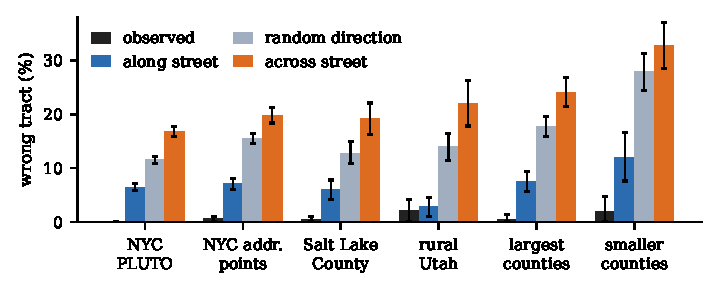
\includegraphics[width=\textwidth]{figures/fig3_direction_test.pdf}
\caption{Near-line addresses with a clear street-segment match (4{,}378, 73\%): observed wrong-tract rate and the same displacement lengths turned along the nearest street, in random directions, or across it (mean of both signs; 95\% bootstrap CIs).}
\label{fig:direction}
\end{figure}

\begin{table}[t]
\centering
\caption{Wrong-tract rate (\%) for near-line addresses, with 95\% CI (Wilson; county-cluster bootstrap for the 18 counties), the rate if every excluded near-line Match were wrong, and the same displacement lengths in random directions.}
\label{tab:real}
\small\setlength{\tabcolsep}{3pt}
\begin{tabular}{lrrrrr}
\toprule
Sample & $n$ & Observed & 95\% CI & Excl.\ as wrong & Random dir. \\
\midrule
NYC, PLUTO reference & 2{,}478 & 0.04 & [0.01, 0.23] & 0.08 & 11.5 \\
NYC, Address Points & 1{,}443 & 0.97 & [0.58, 1.62] & 3.18 & 15.0 \\
Utah, Salt Lake County & 694 & 0.72 & [0.31, 1.68] & 0.86 & 11.7 \\
Utah, six rural counties & 591 & 2.03 & [1.17, 3.52] & 5.39 & 10.8 \\
18 sampled counties & 765 & 1.57 & [0.67, 2.67] & 3.95 & 20.2 \\
\midrule
All & 5{,}971 & 0.74 & [0.55, 0.99] & 1.97 & 13.4 \\
\bottomrule
\end{tabular}
\end{table}

\textbf{Real errors are large but rarely change the tract.} Median displacement is 19--26\,m in NYC, 27--31\,m in Utah and 30--86\,m in the sampled counties, yet near-line rates are 0.04--2.03\% against 10.8--20.2\% for random directions (Table~\ref{tab:real}). The gap survives sensitivity checks: counting every excluded near-line Match as wrong gives at most 5.4\% (rural Utah, against 10.8\%); the observed rate is below the random-direction rate in each of the 18 counties and in every distance band (0--10\,m: 1/52 against 28.0\%; within 100\,m, both strata: 0.70\% against 11.3\%). The tract the geocoder itself returns equals our PIP label for 5{,}970 of 5{,}971 addresses. The two NYC references differ about 24-fold (0.04\% vs.\ 0.97\%): lot points and address points place the same address differently, so the reference source matters as much as the geocoder, and only 13 addresses occur in both samples.

\textbf{Mechanism: direction and the matched block face.} Turning each real displacement along the nearest street gives 6.7\% [6.2, 7.2] wrong tracts, random directions 13.7\% and across the street 19.0\%, with this ordering in all six samples (Fig.~\ref{fig:direction}); direction matters, but along-street movement alone leaves rates far above the observed 0.37\%. The geocoder's own output explains the rest. Every geocode lies on the side of the matched TIGER edge that the geocoder reports, 6.37\,m (median; 99.98\% within 5--8\,m) from it, and TIGER address ranges locate an address to the area on that side of the street~\cite{censusaddr}. When the reference point lies on the matched block face (projecting onto the matched edge, on the reported side, within 60\,m), the tract was wrong for 2 of 5{,}594 near-line addresses (0.04\%). The other 42 errors arise when the reference lies beyond the end of the matched edge (13/168), across it (4/13) or more than 60\,m away (25/112), i.e.\ when the geocoder matched a neighbouring or different block face. Re-placing each geocode at random positions along its own matched edge on the reported side gives 0.88\%, close to the observed 0.75\%, but 63.7\% on the opposite side. Positional spread along the face is thus nearly harmless; tract errors are matching errors. Finer units follow the same pattern: near-line addresses were in the wrong block group for 0.84\% and the wrong block for 1.66\% [1.36, 2.01], against 14.8\% and 22.1\% for random directions; on the matched face 6 of 5{,}594 blocks were wrong, off it 92 of 293. Our rates are lower than earlier tract-error estimates~\cite{brokamp2018,whitsel2006}, partly because only matched addresses are scored and references are address points.

\textbf{Screening at assignment time.} Since geocodes sit 6.4\,m from a street that is often the tract line (95.5\% of the sampled near-line locations), $d_{\mathrm{obs}}$ is weakly informative: abstaining when $d_{\mathrm{obs}}<7$\,m withholds 65\% of near-line addresses and catches 26 of 44 errors, leaving 0.86\% risk among answered ones against 0.74\% without screening; boundary type taken from the geocode, alone or combined with distance in held-out regions, adds at most one error. The geocoder's match details are more informative. Non\_Exact matches (50.4\%) contained 30 errors (odds ratio stratified by region 3.3, $p$=0.003), but 2{,}637 of them differ from the input only in city name (17 errors). Comparing the matched with the input address is sharper: a changed street direction (268 addresses, 11 errors, 4.1\%) or house number (6, 1 error) flags 4.6\% and catches 12 errors, against 5 for distance at the same share; 10 of the 12 are in rural Utah (e.g., N Main St matched to S Main St), so this flag is exploratory. Rates were higher in the smaller sampled counties (2.97\%, 7/236) and rural Utah (2.03\%); near non-street lines (rivers, rail, municipal limits) the rate was 1.9\% (5/266) against 0.68\% (OR 2.8, $p$=0.045; $p$=0.18 without NYC).

\textbf{Program eligibility.} 18.8\% of near-line addresses lie in HUD 2026 Qualified Census Tracts~\cite{hudqct}, which steer Low-Income Housing Tax Credit allocations; 8 of the 44 near-line wrong tracts, and 2 of the 18 in the random stratum, changed this status.

\textbf{Pitfall: generalized boundary files.} Census cartographic boundary files are documented as unsuitable for geocoding or precise area relationships~\cite{censuscb}. Applied to exact benchmark locations (which over-sample boundaries), the 1:500k tract file disagrees with TIGER/Line for 1.64\% [1.32, 2.03] of locations and leaves a further, disjoint 2.3\% outside every polygon; county files disagree for 2.1\% (1:500k), 8.0\% (1:5m) and 15.0\% (1:20m).

%=====================================================================
\section{Implications, Limitations and Conclusion}
\begin{table}[t]
\centering
\caption{Practitioner decision table.}
\label{tab:guide}
\small\setlength{\tabcolsep}{3pt}
\begin{tabular}{L{3.4cm}L{8.2cm}}
\toprule
Situation & Recommendation \\
\midrule
Any area assignment & Use full-resolution TIGER/Line boundaries; cartographic files are for small-scale mapping. \\
Census geocodes & Do not set $R$ from displacement (median 19--86\,m) or flag by $d_{\mathrm{obs}}$; near-line error was 0.04--2.0\% (Table~\ref{tab:real}). Review matches whose street direction or house number differs from the input; Non\_Exact alone mostly flags city-name differences. \\
Smaller or rural counties; non-street lines & Higher observed rates (2.0--3.0\%; 1.9\% near non-street lines, exploratory) and lower match yield: check representativeness. \\
Bounded error of known $R$ & $d_{\mathrm{obs}}\ge R$ guarantees the answer. \\
Gaussian or other unbounded error & Treat $R$ as a percentile; set $\tau$ on held-out data with a location-level (heuristic) bound; overlays add little coverage here. \\
\bottomrule
\end{tabular}
\end{table}

\textbf{Practical guidance} is condensed in Table~\ref{tab:guide}. \textbf{Limitations.} We study one geocoder, whose block-face matching produces the protection we observe; geocoders that place points at parcels or rooftops, or without side offsets, may behave differently, and testing a second geocoder is the main next step. Reference coordinates have their own placement error, counties were chosen by address-database coverage, and samples over-represent boundaries, so rates are not prevalence estimates. Only matched addresses are scored, and yields were lower in rural and smaller counties~\cite{oliver2005}. With 44 near-line errors, flag comparisons are exploratory; the block-face classification uses a 60\,m threshold, and the simulation assumes isotropic error of known scale.

\textbf{Conclusion.} For Census Bureau geocodes, large positional errors rarely change the tract because the coordinate is interpolated along the matched block face and kept on its side of the street, where tract lines usually run; the remaining errors come from matching the wrong block face, which boundary distance detects poorly and a changed street direction or house number in the matched address detects better. Isotropic error models, and distance-to-boundary rules derived from them, overstate wrong-tract risk for this geocoder by an order of magnitude, although under isotropic error a distance rule matches probabilistic overlays at a fraction of the cost. Generalized boundary files remain an avoidable source of error. Reporting uncertain assignments rather than silently choosing one is a low-cost step toward more reliable government statistics and services.

\textbf{Data and code availability.} Benchmark, code and all result tables: \url{https://anonymous.4open.science/r/boundarybench-4678/}. % CAMERA-READY: public repository URL + archive DOI

%=====================================================================
\begin{thebibliography}{99}
\bibitem{censusgeocoder} U.S. Census Bureau: Census Geocoder, \url{https://geocoding.geo.census.gov/}. Accessed Nov 2026
\bibitem{censusgeodoc} U.S. Census Bureau: Census Geocoding Services, \url{https://www.census.gov/data/developers/data-sets/Geocoding-services.html}. Accessed Nov 2026
\bibitem{censuscb} U.S. Census Bureau: Cartographic Boundary File Description, \url{https://www.census.gov/programs-surveys/geography/technical-documentation/naming-convention/cartographic-boundary-file.html}. Accessed Nov 2026
\bibitem{censusaddr} U.S. Census Bureau: Understanding Census Bureau Address Ranges (2016), \url{https://www.census.gov/newsroom/blogs/research-matters/2016/04/understanding-census-bureau-address-ranges.html}. Accessed Nov 2026
\bibitem{tiger2025} U.S. Census Bureau: TIGER/Line Shapefiles 2025, \url{https://www.census.gov/geographies/mapping-files/time-series/geo/tiger-line-file.html}. Accessed Nov 2026
\bibitem{nad} U.S. Department of Transportation: National Address Database, \url{https://www.transportation.gov/gis/national-address-database}. Accessed Nov 2026
\bibitem{berg2026} Berg, A., Gutmann, M., Leyk, S., Kwon, H.: Why it's so hard to match residence addresses to census blocks---and how to fix it. Trans. GIS \textbf{30}(2), e70225 (2026)
\bibitem{blakemore1984} Blakemore, M.: Generalisation and error in spatial data bases. Cartographica \textbf{21}(2--3), 131--139 (1984)
\bibitem{cayo2003} Cayo, M.R., Talbot, T.O.: Positional error in automated geocoding of residential addresses. Int. J. Health Geogr. \textbf{2}, 10 (2003)
\bibitem{brokamp2018} Brokamp, C., Wolfe, C., Lingren, T., Harley, J., Ryan, P.: Decentralized and reproducible geocoding and characterization of community and environmental exposures for multisite studies. J. Am. Med. Inform. Assoc. \textbf{25}(3), 309--314 (2018)
\bibitem{cheung2004} Cheung, C.K., Shi, W., Zhou, X.: A probability-based uncertainty model for point-in-polygon analysis in GIS. GeoInformatica \textbf{8}(1), 71--98 (2004)
\bibitem{chow1970} Chow, C.K.: On optimum recognition error and reject tradeoff. IEEE Trans. Inf. Theory \textbf{16}(1), 41--46 (1970)
\bibitem{geifman2017} Geifman, Y., El-Yaniv, R.: Selective classification for deep neural networks. In: Advances in Neural Information Processing Systems 30, pp. 4878--4887 (2017)
\bibitem{goldberg2012} Goldberg, D.W., Cockburn, M.G.: The effect of administrative boundaries and geocoding error on cancer rates in California. Spat. Spatiotemporal Epidemiol. \textbf{3}(1), 39--54 (2012)
\bibitem{goldberg2007} Goldberg, D.W., Wilson, J.P., Knoblock, C.A.: From text to geographic coordinates: the current state of geocoding. URISA J. \textbf{19}(1), 33--46 (2007)
\bibitem{guo2017} Guo, C., Pleiss, G., Sun, Y., Weinberger, K.Q.: On calibration of modern neural networks. In: Proc. ICML, pp. 1321--1330 (2017)
\bibitem{heuvelink1998} Heuvelink, G.B.M.: Error Propagation in Environmental Modelling with GIS. Taylor \& Francis, London (1998)
\bibitem{hudqct} U.S. Department of Housing and Urban Development: Qualified Census Tracts 2026, \url{https://www.huduser.gov/portal/datasets/qct.html}. Accessed Nov 2026
\bibitem{jacquez2012} Jacquez, G.M.: A research agenda: does geocoding positional error matter in health GIS studies? Spat. Spatiotemporal Epidemiol. \textbf{3}(1), 7--16 (2012)
\bibitem{kinnee2020} Kinnee, E.J., Tripathy, S., Schinasi, L., Shmool, J.L.C., Sheffield, P.E., Holguin, F., Clougherty, J.E.: Geocoding error, spatial uncertainty, and implications for exposure assessment and environmental epidemiology. Int. J. Environ. Res. Public Health \textbf{17}(16), 5845 (2020)
\bibitem{krieger2001} Krieger, N., Waterman, P., Lemieux, K., Zierler, S., Hogan, J.W.: On the wrong side of the tracts? Evaluating the accuracy of geocoding in public health research. Am. J. Public Health \textbf{91}(7), 1114--1116 (2001)
\bibitem{krieger2002} Krieger, N., Chen, J.T., Waterman, P.D., Soobader, M.J., Subramanian, S.V., Carson, R.: Geocoding and monitoring of US socioeconomic inequalities in mortality and cancer incidence: does the choice of area-based measure and geographic level matter? Am. J. Epidemiol. \textbf{156}(5), 471--482 (2002)
\bibitem{oliver2005} Oliver, M.N., Matthews, K.A., Siadaty, M., Hauck, F.R., Pickle, L.W.: Geographic bias related to geocoding in epidemiologic studies. Int. J. Health Geogr. \textbf{4}, 29 (2005)
\bibitem{perkal1958} Perkal, J.: O d{\l}ugo\'sci krzywych empirycznych (On the length of empirical curves). Zastosowania Matematyki \textbf{3}(3--4), 258--284 (1958)
\bibitem{rushton2006} Rushton, G., Armstrong, M.P., Gittler, J., Greene, B.R., Pavlik, C.E., West, M.M., Zimmerman, D.L.: Geocoding in cancer research: a review. Am. J. Prev. Med. \textbf{30}(2S), S16--S24 (2006)
\bibitem{shi2010} Shi, W.: Principles of Modeling Uncertainties in Spatial Data and Spatial Analyses. CRC Press, Boca Raton (2010)
\bibitem{strickland2007} Strickland, M.J., Siffel, C., Gardner, B.R., Berzen, A.K., Correa, A.: Quantifying geocode location error using GIS methods. Environ. Health \textbf{6}, 10 (2007)
\bibitem{zandbergen2008} Zandbergen, P.A.: A comparison of address point, parcel and street geocoding techniques. Comput. Environ. Urban Syst. \textbf{32}(3), 214--232 (2008)
\bibitem{zandbergen2008b} Zandbergen, P.A.: Positional accuracy of spatial data: non-normal distributions and a critique of the national standard for spatial data accuracy. Trans. GIS \textbf{12}(1), 103--130 (2008)
\bibitem{zandbergen2009} Zandbergen, P.A.: Geocoding quality and implications for spatial analysis. Geogr. Compass \textbf{3}(2), 647--680 (2009)
\bibitem{whitsel2006} Whitsel, E.A., Quibrera, P.M., Smith, R.L., Catellier, D.J., Liao, D., Henley, A.C., Heiss, G.: Accuracy of commercial geocoding: assessment and implications. Epidemiol. Perspect. Innov. \textbf{3}, 8 (2006)
\bibitem{wilson2024} Wilson, N.E., Hankinson, M., Magazinnik, A., Sands, M.: Inaccuracies in low income housing geocodes: when and why they matter. Urban Aff. Rev. \textbf{60}(1), 217--231 (2024)
\bibitem{zimmerman2007} Zimmerman, D.L., Fang, X., Mazumdar, S., Rushton, G.: Modeling the probability distribution of positional errors incurred by residential address geocoding. Int. J. Health Geogr. \textbf{6}, 1 (2007)
\end{thebibliography}
\end{document}
